\section{Prior work}

\subsection{Structure editors}
Structure editors provide a way to manipulate the abstract syntax structure of programs directly, in contrast to writing and editing source code of a program in plain text, which also requires a parser to produce an abstract syntax tree. An early example of this is the Cornell Program Synthesizer by Reps and Teitelbaum\cite{timtom81} in 1981.
By using a structure editor, the user can avoid syntax errors and might have a better overview of their source code. Moreover, unfinished blocks of code can be represented by syntactic holes, allowing the programmer to develop a mental model of their code, without getting distracted or blocked by syntax errors.

However structure editors like the Cornell Program Synthesizer\cite{timtom81} allow programmers to create syntactically ill-formed programs. This includes introducing use-before-declaration statements, as the editor cannot manage context-sensitive constraints within the syntax.

In 2017 Omar et al. introduced Hazel\cite{omar}, a programming environment for a functional language with typed holes, which allows for evaluation to continue past holes which might be empty or ill-formed. The motivation for this work is to provide feedback about a program's dynamic behaviour as it is being edited, in contrast to other programming languages and environments which usually only assign dynamic meaning to complete programs. In other words, the Hazel environment\cite{omar} provides feedback on programs, even if they are ill-formed or contain type errors. This is possible by surrounding static and dynamic inconsistencies with typed holes, allowing evaluation to proceed past holes.

The Hazel environment is based on the Hazelnut structure editor calculus, defined by operational semantics, that allow finite edit expressions and inserts holes automatically to guarantee that every editor state has some type.

Hazel itself is not a structure editor, however the core calculus supports incomplete functional programs, also referred to as "holes", which are a central part of the work of Godiksen et. al \cite{godiksen}. They introduced a type-safe structure editor calculus which manipulates a simply-typed lambda calculus with the ability to evaluate programs partially with breakpoints and assign meaning to holes. It also ensures that if an edit action is well-typed, then the resulting program is also well-typed. The editor calculus and programming language have later been used to implement a type-safe structure editor in Elm\cite{KU-bach-missing-ref}.

\subsection{Editor generators}
A common property of the editor calculi and editors mentioned so far is that they are built to work with only one programming language. The calculi are strongly dependent on the language they can manipulate, and if the language were to change, it could require re-writing the complete editor calculus. A solution to this problem is editor generators.

A few years after presenting the Cornell Program Synthesizer, Reps and Teitelbaum also presented The Synthesizer Generator\cite{timtom84} in 1984, which creates structure editors from language descriptions in the form of attribute grammar specifications.

Another example is the Centaur system\cite{centaur}, which takes formalism described in the Metal language\cite{metal}, a collection of concrete syntax, abstract syntax, tree building functions and unparsing (a.k.a. pretty-printing) specifications. The abstract syntax is made of operators and \textit{phyla}, where operators label the nodes of the abstract trees and are either fixed arity or list operators. Operators are defined as having \textit{offsprings}, where fixed-arity operators can have offsprings of different kinds, whereas offsprings of list operators must be of the same kind. This concept is formalized by the concept of \textit{phylum}, where \textit{phyla} (plural of \textit{phylum}) are sets of operators, describing what operators are allowed at every offspring of an operator. In other words, phyla constrain the allowed operators in every subtree of either a non-null fixed arity operator or a list-operator. Each operator-phylum relation is used to maintain syntactically correct trees.
This definition of operators and phyla in Metal strongly relates to Harper's definition of abstract syntax\cite{harper} in the form of sorts, arity-indexed operators and variables. Operators in both definitions represent a node in an abstract syntax tree and having an associated phyla or being arity-indexed serves the same purpose of constraining the possible children of each node, hence maintaining syntactically correct trees.

However, the Centaur system\cite{centaur} lacks a dedicated type-safe editor calculus. Such a type-safe generalized editor calculus has been proposed by \cite{aalborg}, which is a generalization of the work of Godiksen et al. \cite{godiksen}. The generalized editor calculus takes abstract syntax in the form of sorts, arity-indexed operators and variables, as described by Harper\cite{harper}.

\subsection{Partial evaluation}
One of the goals of this project is to implement a generic syntax-directed editor based on the editor calculus proposed by \cite{aalborg}. Implementing such a generic editor relates to the question of how to balance between generality and modularity, brought up by Neil D. Jones\cite{jones-partial-evaluation} in the context of program specialization. If we are presented with a class of similar problems, such as instantiating a syntax-directed editor for different languages, one might consider two extremes: either write many small, but efficient, programs or write a single highly \textit{parametrized} program which can solve any problem.

The first approach is very modular and has the advantage of allowing the programmer to focus solely on performance for every smaller program, but it has an obvious disadvantage of being hard to maintain. Highly modular programming might also lead to performance overhead in terms of passing data back and forth between programs and converting among various internal representations.

The second approach is general and has the advantage of being easier to document and maintain, due to it being a single program. However, it is arguably not well-performing, as some amount of time needs to be spent interpreting the parameters instead of the actual problem-solving computation.

Using a partial evaluator\cite{jones96} to specialize a highly parametrized program into smaller, customized versions, is arguably a better solution than both approaches. This way, only one single program requires maintenance, while allowing it to be specialized, taking advantage of program speedup.

The notion of partial evaluation in terms of program specialization\cite{jones96} includes a partial evaluator, which receives a general program and some static input, resulting in a specialized program that, if specialized in a meaningful way, performs better than the original program. An example provided by Jones is a program computing $x^n$ (program $p$ in listing \ref{lst:jones-ex1}), which can be specialized to having $n = 5$ (program $p_5$ in listing \ref{lst:jones-ex2}), unfolding the recursive calls and reducing $x*1$ to $x$. Formally, the general program $p$ and static input $in_1$ are passed to a partial evaluator $mix$, which outputs a specialized program $p_{in_1}$, which can take dynamic input $in_2$ and produce some output. For an illustration of this example, see figure \ref{fig:partial-eval-ex}.

\begin{lstlisting}[style=inline,label={lst:jones-ex1},caption={Two-input program $p$}]
f(n, x) = if n = 0 then 1
else if even(n) then f (n/2,x)^2
else x * f(n-1,x)
\end{lstlisting}

\begin{lstlisting}[style=inline,label={lst:jones-ex2},caption={Specialization of program $p$}]
f5(x) = x * ((x^2)^2)
\end{lstlisting}

\begin{figure}[H]
    \centering
    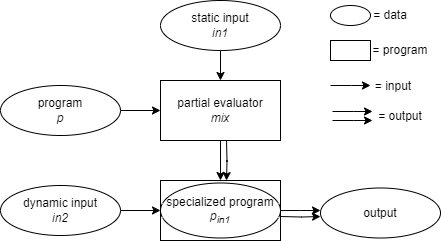
\includegraphics[width=0.75\textwidth]{img/partial-eval.drawio.png}
    \caption{Visualisation of partial evaluation of a two-input program}
    \label{fig:partial-eval-ex}
\end{figure}

This idea of specialization can also be applied to the implementation of this project, where the static input is the syntax of a language, which if partially evaluated with a general program, results in a specialized program. This program represents a syntax-directed editor instance for the static input's language, which can take dynamic input in the form of editor expressions, resulting in either cursor movement or updates to the target language's program. This can be seen as a curried function with following signature:
$$
    f : t_1 \rightarrow t_2 \rightarrow t_3
$$
where $t_1$ is the type of language specifications, $t_2$ is the type of editor expressions and $t_3$ is the type of programs. Given a language specification, $f$ produces a new function $f'$ of type $t_2 \rightarrow t_3$, i.e., a new function that takes an editor expression and returns a program. Here, $f'$ is an instance of the editor for a specific language.

In other words, the implementation can be specialized given some syntax, potentially skipping the process of parsing syntax and generating source code every time a user wishes to use the same editor instance for some language.